%!TEX root = synchrony.tex

\section{Omitted Proofs}

\subsection{Proof of Lemma \ref{imposs:1}} \label{app:imposs:1}
\begin{proof}
\begin{figure}[h]
  \centering
  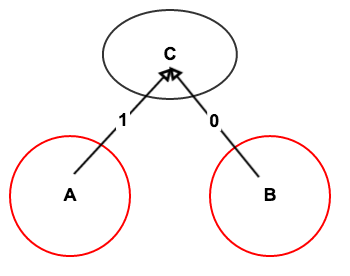
\includegraphics[scale=0.35]{impossible1.png}
  \caption{Case $m \geqslant t$  }
\end{figure}\label{sc1}

%
  The case $n=2$ is trivial. We assume $n \geqslant 3$.
  Suppose that $F$ is a $k$-round interactive consistency algorithm. Since $n \leqslant
  2m+t$, $P$ can be partitioned into three nonempty sets $A$, $B$, and $C$,
  with $| A | \leqslant m$, $| B | \leqslant m$, $| C | \leqslant t$. 
  
  We define two scenarios $\alpha$ and $\beta$.
  In $\alpha$, all processes have 0 as initial values.
  Processes in $B$ are faulty and send  to $C$ processes messages
  pretending that processes in $A$ have 1 as initial value.
  
   In $\beta$, processes in $A$ have 1 as initial value and all  others processes have 0 as initial value.
  Processes in $A$ are faulty and send to $C$ messages 
  pretending that processes in $A$ have 0 as initial value (see Figure~\ref{sc1}).
  
  In the two scenarios, processes in $C$ get the same messages, but in the first scenario 
  they have to decide 0 for processes in $A$ and $1$ in the second scenario leading to a contradiction.
    
More precisely  the scenarios $\alpha$
  and $\beta$ are defined as follows:
  \begin{enumerateroman}
    \item For every $w \in P^{+}$ not starting with a process of $A$, let
    \[ \alpha ( w ) = \beta ( w ) =0. \]
    \item For every $a \in A$, $b \in B$, $c \in C$ let
    \[ \alpha ( a ) = \alpha ( a a )  =  \alpha ( a b ) = \alpha ( a c )  = 0,
    \]
    \[ \beta ( a ) = \beta ( a a ) = \beta ( a b ) =1 \nocomma , \beta ( a c )
       =0. \]
    \item We define this part iteratively. 
    For every $a \in A$, $b \in B$, $c \in C$, $p \in P$, $w \in
    a P^{\ast}$, let
    \[ \alpha ( w c p ) = \alpha ( w c ) \nocomma , \alpha ( w a p ) = \alpha
       ( w a ) , \]
    \[ \beta ( w c p ) = \beta ( w c ) \nocomma , \beta ( w b p ) = \beta ( w
       b ) , \]
    \[ \alpha ( w b c ) = \beta ( w b ) \nocomma , \alpha ( w b a ) = \alpha
       ( w b ) , \]
    \[ \beta ( w a c ) = \alpha ( w a ) , \beta ( w a b )  =  \beta ( w a )
       . \]
  \end{enumerateroman}
  $\alpha$ is a  scenario in which processes in $B$ are faulty 
and  $\beta$ is a  scenario in which  faulty 
  processes are in set $A$. 
 Moreover,  $\alpha_{c} =
  \beta_{c}$ for all $c \in C$ then for any $a \in A$, $c \in C$
   \[ F_c ( \alpha_{c} )[a] = F_c ( \beta_{c} )[a].  \]

But for any $a \in A$, $c \in C$, as $F$ is a $k$-round  interactive consistency algorithm
    \[ F_c ( \alpha_{c})[a] = \alpha ( a ) = 0 , \] 
  \[ F_c ( \beta_{c} )[a] = \beta ( a ) =1 , \]
leading to a contradiction.
\end{proof}

\subsection{Proof of Lemma \ref{imposs:2}}\label{app:imposs:2}

\begin{proof}
\begin{figure}[h]
  \centering
  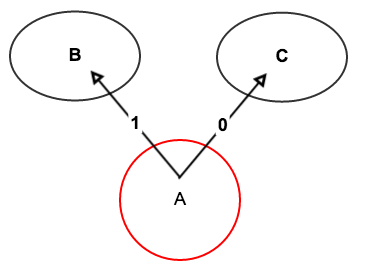
\includegraphics[scale=0.35]{impossible2.png}
  \caption{Case $t \geqslant m$  }
\end{figure}\label{sc2}

  This proof is similar to the proof above. 
  The case $n=2$ is trivial. We assume $n \geqslant 3$.
  Suppose that $F$ is a $k$-round  interactive
  consistency algorithm. Since $n \leqslant 2t+m$, $P$ can be partitioned into
  three non-empty sets $A$, $B$, and $C$, with $| A | \leqslant m$, $| B | \leqslant t$, $| C |
  \leqslant t$. 
  
   We define two scenarios $\alpha$ and $\beta$.
  In $\alpha$, all processes have 0 as initial values.
  Processes in $A$ are faulty and send to processes in $C$  messages
  pretending that they have  1 as initial value. 
  
   In $\beta$, processes in $A$ have 1 as initial value and all  others processes have 0 as initial value.
  Processes in $A$ are faulty and send to processes in $B$ messages 
  pretending that they have 1 as initial value (see Figure~\ref{sc1}).
  
  In the two scenarios, processes in $B$ and $C$  get the same messages, but in the first scenario 
  they have to decide 0 for processes in $A$ and $1$ in the second scenario giving the contradiction.
    
More precisely  the scenarios $\alpha$
  and $\beta$ are defined as follows:
  \begin{enumerateroman}
    \item For every $w \in P^{+}$ not starting with a process of $A$, let
    \[ \alpha ( w ) = \beta ( w ) =0. \]
    \item For every $a \in A$, $b \in B$, $c \in C$ let
    \[ \alpha ( a ) = \alpha ( a a )  =  \alpha ( a b ) =0, \alpha ( a c )  =
       1, \]
    \[ \beta ( a ) = \beta ( a a ) = \beta ( a c ) =1 \nocomma , \beta ( a b )
       =0. \]
    \item We define this part iteratively. For every $a \in A$, $b \in B$, $c \in C$, $p \in P$, $w \in
    a P^{\ast}$, let
    \[ \alpha ( w b p ) = \alpha ( w b ) , \alpha ( w c p ) = \alpha ( w c ) ,
    \]
    \[ \beta ( w b p ) = \beta ( w b ) \nocomma , \beta ( w c p ) =\beta ( w c ) ,
    \]
    \[ \alpha ( w a b ) = \alpha ( w a ) \nocomma , \beta ( w a c ) = \beta (
       w a ) , \]
    \[ \alpha ( w a c ) = \beta ( w a ) \nocomma , \beta ( w a b ) = \alpha
       ( w a ) . \]
  \end{enumerateroman}
 $\alpha$ and $\beta$ are scenarios in which processes in $A$ are faulty.
  Moreover, $\alpha_{b} =
  \beta_{b}$, $\alpha_{c} = \beta_{c}$ for all $b \in B$ and $c \in C$. 
  Then for any $a \in A$, $b \in B$:
   \[ F_b ( \alpha_{b} )[a] =F_b ( \beta_{b} )[a]. \]

  
But for any $a \in A$, $b \in B$, as $F$ is a $k$-round  interactive consistency algorithm
  \[ F_b ( \alpha_{b} )[a] = \alpha ( a )
     =0, \]
       \[ F_b ( \beta_{b} )[a] = \beta ( a )
     =1, \]
  leading to the contradiction.
\end{proof}

\subsection{Proof of Lemma \ref{imposs:3}} \label{app:imposs:3}

\begin{proof}
  Suppose that $F$ is a $k$-round  interactive consistency algorithm. 
  
  Since $n \leqslant
  m+2t$, $P$ can be partitioned into three nonempty sets $A$, $B$, and $C$,
  with $| A | \leqslant m$, $| B | \leqslant t$, $| C | \leqslant t$. 
  
   We define two scenarios $\alpha$ and $\beta$.
  In $\alpha$, all processes have 0 as initial values.
  Processes in $A$ are faulty and send  to processes in $C$  messages
  pretending that they have  1 as initial value. 
  
   In $\beta$, processes in $A$ have 1 as initial value and all  others processes have 0 as initial value.
  Processes in $A$ are faulty and send to processes in $B$ messages 
  pretending that they have 1 as initial value.
  

  
    In the two scenarios, processes in $B$ and $C$  get the same messages, but in the first scenario $\alpha$
  they have to decide 0 for processes in $A$ and $1$ in the second scenario giving the contradiction.
  
  We
  define scenarios $\alpha$ and $\beta$ as follows:
  \begin{enumerateroman}
    \item For every $w \in P^{+}$ not starting with a member of $A$, let
    \[ \alpha ( w ) = \beta ( w ) =0. \]
    \item For every $a_{1}  \in A^{+}$, $a \in A,b \in B,c
    \in C$, $w \in P^{\ast}$, let
    \[ \alpha ( a ) =0, \beta ( a ) =1, \]
    \[ \alpha ( a_{1}  b w ) = \beta ( a_{1}  b w ) =0, \]
    \[ \alpha ( a_{1}  c w ) = \beta ( a_{1}  c w ) =1. \]
    \item All other messages are sent and forwarded based on these messages
    correctly.
  \end{enumerateroman}
  
  $\alpha$ and $\beta$ are scenarios in which processes in $A$ are faulty.
  Moreover, $\alpha_{b} =
  \beta_{b}$, $\alpha_{c} = \beta_{c}$ for all $b \in B$ and $c \in C$. 
  Then for any $a \in A$, $b \in B$:
   \[ F_b ( \alpha_{b} )[a] =F_b ( \beta_{b} )[a]  \]

  
But for any $a \in A$, $b \in B$, as $F$ is a $k$-round  interactive consistency algorithm
  \[ F_b ( \alpha_{b} )[a] = \alpha ( a )
     =0, \]
       \[ F_b ( \beta_{b} )[a] = \beta ( a )
     =1, \]
  leading to a contradiction.
%  Note that, the only difference of $\alpha$ and $\beta$ is the initial value
%  of $A$. We can easy check that $A$ only lies to $B$ ($C$ resp.) for scenario
%  $\alpha$ ($\beta$ resp.). So it is impossible for $B$ or $C$ to tell the
%  real initial value of $A$ in these two scenarios.
\end{proof}

